\documentclass[a4paper,11pt,fleqn,twocolumn,twoside,dvipdfmx]{scrartcl}
\usepackage[utf8]{inputenc}
\usepackage[T1]{fontenc}
\usepackage[ngerman]{babel}
\usepackage{microtype}
\usepackage{amsmath}
\usepackage{amssymb}
\usepackage{lipsum}

\usepackage{libertine}
\usepackage[libertine]{newtxmath}
\addtokomafont{disposition}{\rmfamily}

\usepackage{booktabs}
\usepackage{graphicx}
\numberwithin{equation}{section}

\usepackage{geometry}
\geometry{a4paper,left=25mm,right=12mm,top=24mm,bottom=28mm}
\setlength{\columnsep}{5mm}

\usepackage[colorlinks=true,linkcolor=black]{hyperref}

\usepackage{lastpage}
\usepackage[automark]{scrlayer-scrpage}
\ohead{}
\ihead{}
\chead{}
\cfoot{\normalfont{\pagemark} von {\pageref{LastPage}}}
\ofoot{}

\newcommand{\ee}{\mathrm e}
\newcommand{\ui}{\mathrm i}
\newcommand{\real}{\operatorname{Re}}
\newcommand{\imag}{\operatorname{Im}}
\newcommand{\uv}[1]{\underline{#1}}
\newcommand{\bv}[1]{\mathbf{#1}}

\newcommand{\N}{\mathbb N}
\newcommand{\Z}{\mathbb Z}
\newcommand{\Q}{\mathbb Q}
\newcommand{\R}{\mathbb R}
\newcommand{\C}{\mathbb C}

\newcommand{\id}{\operatorname{id}}
\newcommand{\sgn}{\operatorname{sgn}}
\newcommand{\Abb}{\operatorname{Abb}}
\newcommand{\unit}[1]{\mathrm{#1}}
\newcommand{\chem}[1]{\mathrm{#1}}
\newcommand{\strong}[1]{\textbf{#1}}

\begin{document}

\noindent
{\Large\textbf{Epidemiologische Betrachtungen\\
zur Covid-19-Pandemie 2020}}\\[4pt]
4. März 2020

\tableofcontents

\section{Theorie}

\subsection{Die Reproduktionszahl}

Die \emph{Basisreproduktionszahl} $R_0$ ist die Anzahl der Individuen,
die ein infiziertes Individuum im Mittel infiziert. Die tatsächliche
Anzahl wird allerdings durch die \emph{Nettoreproduktionszahl}%
\begin{equation}\label{eq:Nettoreproduktionszahl}
R_q = R_0(1-q).
\end{equation}
beschrieben. Hierbei ist $q$ der immune Anteil der Bevölkerung.
Damit die Epedemie zum Stillstand kommt, muss $R_q<1$ sein.
Aus dem Ansatz $R_q=1$ ergibt sich%
\begin{equation}
q_c := q = 1-\frac{R_q}{R_0} = 1-\frac{1}{R_0}.
\end{equation}
Ist dieser Anteil $q_c$ der Bevölkerung immun, bricht die Epidemie
also gar nicht erst aus. Man spricht von der
\emph{kritischen Immunisierungsschwelle} oder \emph{Schwelle
zur Herdenimmunität}.

Für bestimmte Krankheiten lässt sich $R_0$ abschätzen, wobei
dieser Wert allerdings empfindlich vom Verhalten der Bevölkerung und
eventueller Quarantäne abhängt.


\subsection{Das SIR-Modell}

Die Bevölkerung wird aufgeteilt in die Anteile $S,I,R$. Hierbei sind
$S$ die Anfälligen (engl. susceptibles), $I$ die Infizierten (engl.
infected) und $R$ die Erholten (engl. recovered). Die Anteile
$S,I,R$ sind normiert, so dass $S+I+R=1$ gilt. Die absolute Zahl
ergibt sich durch Multiplikation des jeweiligen Anteils mit der
Bevölkerungszahl $N$.

In einem Zeitschritt von $t$ zu $t+h$ mit $h:=\Delta t$ wird es zu
einer Zunahme von $I$ kommen. Diese Zunahme ist zunächst davon
abhängig, wie
viele Infizierte $I$ und Anfällige $S$ es gerade gibt. Sei
$S$ fest. Gäbe es zwischen den Anfälligen doppelt so viele Infizierte,
würde dies zu der doppelten Zunahme führen. Sei nun umgekehrt $I$
fest. Gäbe es nur halb so viele Anfällige, wäre es nur halb so
wahrscheinlich, dass ein Infizierter einen Anfälligen infiziert.
Demnach sollte die Zunahme proportional zu $I$ und $S$ sein, also
zum Produkt $IS$. Die Proportionalitätskonstante sei $\beta$. Wir machen
also den Ansatz%
\begin{equation}
I_{t+h} = I_t + h\beta I_t S_t.
\end{equation}
Man kann auch $h=1$ setzen. Für die Anfälligen gilt dementsprechend
$S_{t+h}=S_t-h\beta I_t S_t$. Nun muss man schließlich noch beachten,
dass sich Infizierte mit der Zeit erholen. Die Abnahme der Infizierten
ist proportional zur Zahl der Infizierten, unter der Annahme dass
die Zahl aus Altinfektionen und Neuinfektionen besteht. Die
Proportionalitätskonstante sei $\gamma$.
Nun ergibt sich insgesamt das Modell%
\begin{align}
S_{t+h} &= S_t-h\beta I_t S_t,\\
I_{t+h} &= I_t+h\beta I_t S_t-h\gamma I_t,\\
R_{t+h} &= R_t+h\gamma I_t.
\end{align}
Dies ist ein diskretes dynamisches System, gegeben durch ein
nichtlineares System von Differenzengleichungen. Umformung der jeweiligen
Gleichung bringt%
\begin{align}
\frac{S_{t+h}-S_t}{h} &= -\beta I_t S_T\\
\frac{I_{t+h}-I_t}{h} &= \beta I_t S_t-\gamma I_t,\\
\frac{R_{t+h}-R_t}{h} &= \gamma I_t.
\end{align}
Für $h\to 0$ ergibt sich
\begin{align}
S' &= -\beta IS,\\
I' &= \beta IS-\gamma I,\\
R' &= \gamma I.
\end{align}
Dies ist ein kontinuierliches dynamisches System, gegeben durch ein
nichtlineares System von Differentialgleichungen. Aufgrund von
$S+I+R=1$ gilt%
\begin{equation}
S'+I'+R'=0.
\end{equation}
Man bezeichnet $\beta$ als \emph{Erkrankungsrate} und
$\gamma$ als \emph{Gesundungsrate}.

Angenommen es ist $I\approx 0$, aber $I>0$. Unter welchem Umstand
gibt es dann keine Neuerkrankungen? Dazu muss $I'=0$ sein. Dieser
Ansatz führt zu%
\begin{equation}
0 = \beta IS-\gamma I \Leftrightarrow 0 = \beta S-\gamma
\Leftrightarrow S = \frac{\gamma}{\beta}.
\end{equation}
Aufgrund von $R+S\approx 1$ ist $q=R=1-S$. Einsetzen von
$q$ in Gleichung \eqref{eq:Nettoreproduktionszahl} bringt%
\begin{equation}
R_q = R_0(1-q) = R_0 S = R_0\frac{\gamma}{\beta}.
\end{equation}
Weil $R_q=1$ sein muss, ergibt sich die Beziehung%
\begin{equation}
R_0 = \frac{\beta}{\gamma}.
\end{equation}
Interessant ist nun das Grenzverhalten
\begin{equation}
R(\infty) := \lim_{t\to\infty} R(t),
\end{equation}
das eine Aussage macht, wie viele Individuen die Erkrankung bei
Abwesenheit von Quarantäne durchmachen werden. Wie sich aus einer
numerischen Simulation ergibt, führt ein
Startzustand $S\approx 1$ und $I\approx 0$ zu $R(\infty)>q$. Bei $R_0=3$
ist z.\,B. $R(\infty)=94\,\%$, obwohl $q=66\,\%$ ist. Siehe Abb.
\ref{fig:R0-drei}.


\subsection{Ermittlung der Modellparameter}

Für das SIR"=Modell sind die Parameter sicherlich bestimmbar,
indem die numerische Lösung mit Messdaten verglichen wird.
Variation der Parameter $\beta$ und $\gamma$ führt zu unterschiedlichen
Fehlerquadratsummen, von diesen wird die minimale ermittelt.

Unabhängig vom genannten Ansatz folgen noch analytische Betrachtungen,
womit sich die Parameter unter Umständen mit weniger Aufwand ermitteln
lassen.

Am Anfang steigt die Zahl der Infektionen exponentiell. Die Kurve
$I(t)$ ist in dieser Phase also beschrieben durch
$I=I_0\ee^{\lambda t}$, wobei man $\lambda$ nach Linearisierung aus
einer Regression ermitteln kann. Es gilt $I'=\lambda I$. Für die
Dgl. ergibt sich die Faktorisierung%
\begin{equation}
I' = \beta IS-\gamma I = (\beta S-\gamma)I.
\end{equation}
Am Anfang der Phase ist in guter Näherung $S\approx 1$, vor allem bei
großer Bevölkerungszahl. Demnach gilt%
\begin{equation}
\lambda = \beta-\gamma.
\end{equation}
Setzt man $\gamma=\beta/R_0$ ein, gelangt man zu
\begin{equation}
\lambda = \beta\Big(1-\frac{1}{R_0}\Big) = \beta q_c.
\end{equation}

\clearpage
\onecolumn
\section{Abbildungen}

\begin{figure}[h]
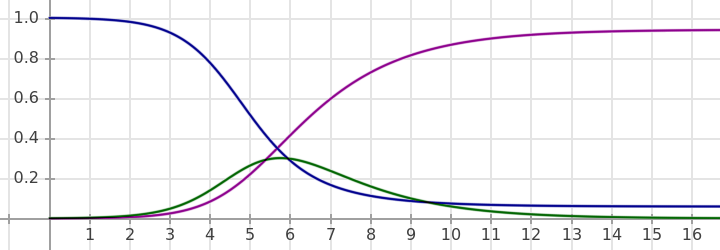
\includegraphics[width=14cm]{img/SIR-Simulation-R0-drei.png}
\caption{Simulation zum SIR-Modell.
$S$ in blau, $I$ in grün, $R$ in magenta.\;\;%
(\href{https://cas-de.github.io/plot.htm?S(t),I(t),R(t);%
\%20\%5bS,I,R\%5d\%27=\%5b-beta*I*S,beta*I*S-gamma*I,gamma*I\%5d;%
\%20p:=\%5b0,0.999,0.001,0\%5d;\%20gamma:=beta/3;\%20beta:=2;%
\%20tw(0,40);;scale(1,0.2),P(10.2,0.5)}{$\rightarrow$Link})%
\newline
Anfangswerte: $S:=0.999,I:=0.001,R:=0$.\newline
Parameter: $\beta:=2$ und $\gamma:=\beta/R_0$ mit $R_0:=3$.}
\label{fig:R0-drei}
\end{figure}



\end{document}
